\begin{figure}[h!]
\begin{center}
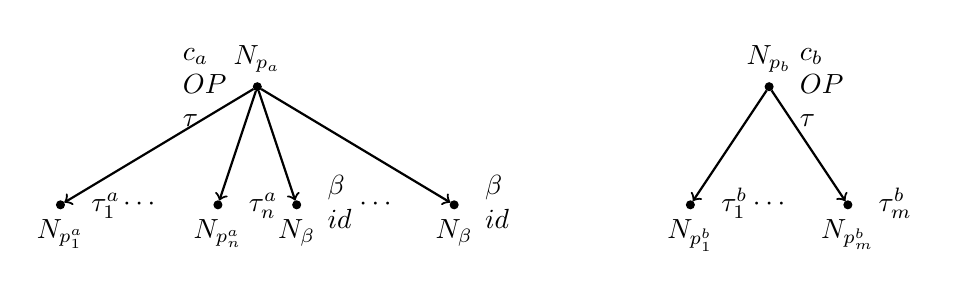
\begin{tikzpicture}[yscale=-1,
place/.style={circle,draw=black, fill=black, inner sep=0pt, 
              minimum size=1mm}]

  \node[place] (1st) at (2.5, 0) [label=above: $N_{p_a}$,
                                label=left: 
    \begin{tabular}{l}
      $c_a$\\
      $OP$\\
      $\tau$\\ 
    \end{tabular}
] {};
  \node[place] (2nd) at (0, 1.5) [label=below:  $N_{p_1^a}$,
  	label=right:
    		\begin{tabular}{l}
    			 $\tau_1^a$\\ 
   		 \end{tabular} ] {};
  \node[place] (3rd) at (2, 1.5) [label=below:   $N_{p_n^a}$,    
  	label=right:   
   		\begin{tabular}{l}
       			$\tau_n^a$\\ 
    		\end{tabular}] {}; 
  \node[place] (4th) at (3, 1.5) [label=below:  $N_{\beta}$,
  	label=right:
  	\begin{tabular}{l}
     		$\beta$\\
     		$id$\\ 
    	\end{tabular}] {}; 
  \node[place] (5th) at (5, 1.5) [label=below:  $N_{\beta}$,
  label=right:
  	\begin{tabular}{l}
     		$\beta$\\
     		$id$\\ 
    	\end{tabular}] {}; 
  
  \node (dots) at (1,1.5) {$\cdots$};
  \node (dots) at (4,1.5) {$\cdots$};
	
  \draw[->, thick] (1st) -- (2nd);
  \draw[->, thick] (1st) -- (3rd);
  \draw[->, thick] (1st) -- (4th);
  \draw[->, thick] (1st) -- (5th);


\begin{scope}[xshift=8cm]
  \node[place] (1st) at (1, 0) [label=above: $N_{p_b}$,
                                label=right: 
       \begin{tabular}{l}
         $c_b$\\
         $OP$\\
         $\tau$\\
       \end{tabular}
] {};
  \node[place] (2nd) at (0, 1.5) [label=below:  $N_{p_1^b}$,
  label=right:
  \begin{tabular}{l}
     $\tau_1^b$\\ 
    \end{tabular}]{};
  \node[place] (3rd) at (2, 1.5) [label=below:  $N_{p_m^b}$,
  label=right:
  \begin{tabular}{l}
     $\tau_m^b$\\ 
    \end{tabular}] {}; 

  \node (dots) at (1,1.5) {$\cdots$};
	
  \draw[->, thick] (1st) -- (2nd);
  \draw[->, thick] (1st) -- (3rd);
\end{scope}

);
\end{tikzpicture}
\end{center}
\caption{Comparison between two complex predicates} 
\label{fig:SimCC}
\end{figure}